\documentclass{article}

\usepackage{fancyhdr}
\usepackage{extramarks}
\usepackage{amsmath}
\usepackage{amsthm}
\usepackage{amsfonts}
\usepackage{tikz}
\usepackage[plain]{algorithm}
\usepackage{algpseudocode}
\usepackage{graphicx}
\usepackage{wrapfig}
\usepackage{url}
\usepackage{wrapfig}
\usepackage{color}
\usepackage{marvosym}
\usepackage{enumerate}
\usepackage{subfigure}
\usepackage{tikz}
\usepackage{amsmath}
\usepackage{amssymb}
\usepackage{hyperref}
\usepackage{bm}
\usepackage{graphicx}

\usetikzlibrary{automata,positioning}

%
% Basic Document Settings
%

\topmargin=-0.45in
\evensidemargin=0in
\oddsidemargin=0in
\textwidth=6.5in
\textheight=9.0in
\headsep=0.25in

\linespread{1.1}

\pagestyle{fancy}
\lhead{\hmwkAuthorName}
\chead{\hmwkClass\ (\hmwkClassInstructor\ \hmwkClassTime): \hmwkTitle}
\rhead{\firstxmark}
\lfoot{\lastxmark}
\cfoot{\thepage}

\renewcommand\headrulewidth{0.4pt}
\renewcommand\footrulewidth{0.4pt}

\newcommand*{\Scale}[2][4]{\scalebox{#1}{$#2$}}%
\newcommand*{\Resize}[2]{\resizebox{#1}{!}{$#2$}}%

\setlength\parindent{0pt}

%
% Create Problem Sections
%

\newcommand{\enterProblemHeader}[1]{
    \nobreak\extramarks{}{Problem \arabic{#1} continued on next page\ldots}\nobreak{}
    \nobreak\extramarks{Problem \arabic{#1} (continued)}{Problem \arabic{#1} continued on next page\ldots}\nobreak{}
}

\newcommand{\exitProblemHeader}[1]{
    \nobreak\extramarks{Problem \arabic{#1} (continued)}{Problem \arabic{#1} continued on next page\ldots}\nobreak{}
    \stepcounter{#1}
    \nobreak\extramarks{Problem \arabic{#1}}{}\nobreak{}
}

\setcounter{secnumdepth}{0}
\newcounter{partCounter}
\newcounter{homeworkProblemCounter}
\setcounter{homeworkProblemCounter}{1}
\nobreak\extramarks{Problem \arabic{homeworkProblemCounter}}{}\nobreak{}

%
% Homework Problem Environment
%
% This environment takes an optional argument. When given, it will adjust the
% problem counter. This is useful for when the problems given for your
% assignment aren't sequential. See the last 3 problems of this template for an
% example.
%
\newenvironment{homeworkProblem}[1][-1]{
    \ifnum#1>0
        \setcounter{homeworkProblemCounter}{#1}
    \fi
    \section{Problem \arabic{homeworkProblemCounter}}
    \setcounter{partCounter}{1}
    \enterProblemHeader{homeworkProblemCounter}
}{
    \exitProblemHeader{homeworkProblemCounter}
}

%
% Homework Details
%   - Title
%   - Due date
%   - Class
%   - Section/Time
%   - Instructor
%   - Author
%

\newcommand{\hmwkTitle}{Homework\ \#3}
\newcommand{\hmwkDueDate}{March 26, 2017}
\newcommand{\hmwkClass}{ISyE 6740}
\newcommand{\hmwkClassTime}{}
\newcommand{\hmwkClassInstructor}{Professor Tuo Zhao}
\newcommand{\hmwkAuthorName}{\textbf{Javier Recasens}}


%
% Title Page
%

\title{
    \vspace{2in}
    \textmd{\textbf{\hmwkClass:\ \hmwkTitle}}\\
    \normalsize\vspace{0.1in}\small{Due\ on\ \hmwkDueDate\ at 11:59pm}\\
    \vspace{0.1in}\large{\textit{\hmwkClassInstructor\ \hmwkClassTime}}
    \vspace{3in}
}

\author{\hmwkAuthorName}
\date{}

\renewcommand{\part}[1]{\textbf{\large Part \Alph{partCounter}}\stepcounter{partCounter}\\}

%
% Various Helper Commands
%

% Useful for algorithms
\newcommand{\alg}[1]{\textsc{\bfseries \footnotesize #1}}

% For derivatives
\newcommand{\deriv}[1]{\frac{\mathrm{d}}{\mathrm{d}x} (#1)}

% For partial derivatives
\newcommand{\pderiv}[2]{\frac{\partial}{\partial #1} (#2)}

% Integral dx
\newcommand{\dx}{\mathrm{d}x}

% Alias for the Solution section header
\newcommand{\solution}{\textbf{\large Solution}}

% Probability commands: Expectation, Variance, Covariance, Bias
\newcommand{\E}{\mathrm{E}}
\newcommand{\Var}{\mathrm{Var}}
\newcommand{\Cov}{\mathrm{Cov}}
\newcommand{\Bias}{\mathrm{Bias}}

\newcommand{\vw}{{\bf w}}
\newcommand{\vx}{{\bf x}}
\newcommand{\vy}{{\bf y}}
\newcommand{\vxi}{{\bf x}_i}
\newcommand{\yi}{y_i}
\newcommand{\vxj}{{\bf x}_j}
\newcommand{\vxn}{{\bf x}_n}
\newcommand{\yj}{y_j}
\newcommand{\ai}{\alpha_i}
\newcommand{\aj}{\alpha_j}
\newcommand{\X}{{\bf X}}
\newcommand{\Y}{{\bf Y}}
\newcommand{\vz}{{\bf z}}
\newcommand{\msigma}{{\bf \Sigma}}
\newcommand{\vmu}{{\bf \mu}}
\newcommand{\vmuk}{{\bf \mu}_k}
\newcommand{\msigmak}{{\bf \Sigma}_k}
\newcommand{\vmuj}{{\bf \mu}_j}
\newcommand{\msigmaj}{{\bf \Sigma}_j}
\newcommand{\pij}{\pi_j}
\newcommand{\pik}{\pi_k}
\newcommand{\D}{\mathcal{D}}
\newcommand{\el}{\mathcal{L}}
\newcommand{\N}{\mathcal{N}}
\newcommand{\vxij}{{\bf x}_{ij}}
\newcommand{\vt}{{\bf t}}
\newcommand{\yh}{\hat{y}}
\newcommand{\code}[1]{{\footnotesize \tt #1}}
\newcommand{\alphai}{\alpha_i}
\newcommand{\vect}[1]{\boldsymbol{#1}}
\DeclareMathOperator{\Tr}{Tr}

\begin{document}

\maketitle

\pagebreak

R code for all problems can be found in the Annex.

\begin{homeworkProblem}
  \paragraph{Gradient Descent for Multiple Linear Regression}
  ~\\
 \part
 \item Please write down the gradient $\nabla f(\vect{\beta})$. 
  \\
  
	\solution
     \\
			\[
			\begin{split}
			f(\vect{\beta})
			&=  \frac{1}{2n} \| \vect{Y} - \vect{X}\vect{\beta}\|_2^2
			\\
			&=  \frac{1}{2n} (\vect{Y} - \vect{X}\vect{\beta})^\top (\vect{Y} - \vect{X}\vect{\beta})
			\\
			&=  \frac{1}{2n} \Big(
						\vect{Y}^\top \vect{Y} 
						- \vect{Y}^\top \vect{X}\vect{\beta}
						- \vect{Y}^\top \vect{X}\vect{\beta} 
					    + \vect{\beta}^\top \vect{X}^\top \vect{X} \vect{\beta} 
						\Big)
			\\
			&=  		 \frac{1}{2n} \vect{Y}^\top \vect{Y} 
						- \frac{1}{n} \vect{Y}^\top \vect{X}\vect{\beta}
						+ \frac{1}{2n} \vect{\beta}^\top \vect{X}^\top \vect{X} \vect{\beta} 		
			\end{split}
			\]
     \\
Derivative with respect to $\vect{\beta}$:
     \\
			\[
			\begin{split}
			\nabla f(\vect{\beta})
			&= - \frac{1}{n} \vect{Y}^\top \vect{X} + \frac{1}{n} \vect{X}^\top \vect{X} \vect{\beta}
			\\
			&=  \frac{1}{n} (\vect{X}^\top \vect{X} \vect{\beta} - \vect{X}^\top \vect{Y})
			\\
			&=  \frac{\vect{X}^\top (\vect{X} \vect{\beta} - \vect{Y})	}{n} 
			\end{split}
			\]

\part
\item Please write down the step size you use in every iteration and explain
why you use it.
\\

\solution

$f(\vect{\beta})$ is twice differentiable and its Hessian $\nabla^2 f(\vect{\beta})$ is $\vect{X}^\top\vect{X} / n$, which does not depend on $\vect{\beta}$. Because this cost function is convex we know that its Hessian is positive semidefinite, so we have that (using the definition of greatest curvature):

\begin{equation*}
\begin{aligned}
\vect{0} \leq  \nabla^2 f(\vect{\beta}) \leq \frac 1n \|\vect{X}\|_2 \vect{I}
\end{aligned}
\end{equation*}

Therefore, the smallest Lipschitz constant of $\nabla f$ is the largest eigenvalue of $\frac 1n \vect{X}^\top\vect{X}$. We know that matrix 2-norm induced by the euclidean vector norm is:

\begin{equation*}
\begin{aligned}
\|\vect{X}\|_2
&= \underset{\|\vect{y}\|_2 = 1}{\text{minimize}}
& \|\vect{Ay}\|_2\\
&= \sqrt{{\lambda}_{max}}  \\
\end{aligned}
\end{equation*}

Where ${\lambda}_{max}$ is the largest number $\lambda$ such that $\vect{X}^\top\vect{X} - \lambda\vect{I}$ is singular. i.e. ${\lambda}_{max}$ is the largest eigenvalue of $\vect{X}^\top\vect{X}$.
\\

Since we want to take the biggest steps possible, we can compute the Lipschitz constant as $L = \frac 1n \|\vect{X}\|_2 ^ 2$ and set a fixed step size: 
\[
\begin{split}
\alpha
&= \frac 1L =  \frac{n}{\|\vect{X}\|_2 ^ 2}
\end{split}
\]	
\\

\part
\item Please explain the rule of stopping your gradient descent algorithm.
\\

\solution

In a descent method, as each new point is generated by the algorithm, the corresponding value of the objective function decreases in value. The gradient varies as the search proceeds, tending to zero as we approach the minimizer.
\\
The stopping rules that we will use:

\begin{itemize}
	\item Condition $ \nabla f(\vect{{\beta}}^{(k+1)}) = 0$. However, this condition is not directly suitable as a practical stopping criterion because the numerical computation of the gradient will rarely be identically equal to zero. A practical criterion is to check if the norm $\|\nabla f(\vect{{\beta}}^{(k+1)})\|_2$ is less than a pre-specified threshold. 
	\item Also we will compute $\|f(\vect{{\beta}}^{(k+1)}) - f(\vect{{\beta}}^{(k)}\|$, and if the difference is less than some threshold, then we stop.
	\item Finally, in some cases, to halt numerical algorithms a pre-specified number of iterations need to be specified, so if the above are not met the algorithm will stop after a finite number of iterations.
\end{itemize}
~\\
\part
\item Please draw a plot of $f(\vect{\beta})$ versus number of iterations to demonstrate the convergence of your algorithm.
\\

\solution
\\
After running 50 iterations we plot $f(\beta)$ versus number of iterations. We can see that the convergence of our algorithm is very fast:

\begin{center}
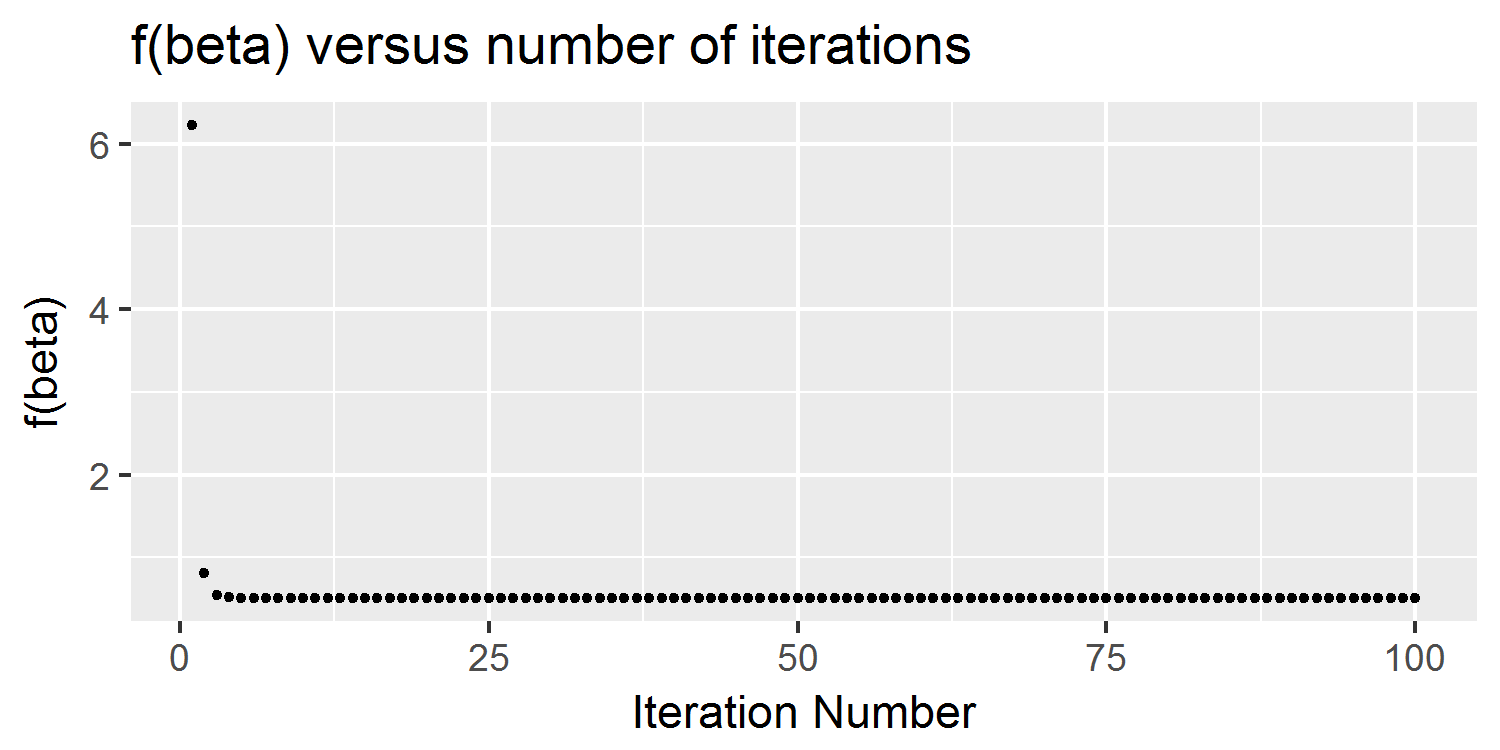
\includegraphics{../R/P1d_Plot}
\end{center}
\part
\item Please compare the result $\beta^*$ returned by your algorithm with the true $\beta$ by computing the mean squared error $\|\beta^* - \beta \|_2^2/30$.
\\

\solution
\\
The mean squared error (MSE) is:

$MSE = \|\beta^* - \beta \|_2^2/30 = 0.0000409143$.

This is a very small MSE which was reached very fast. Our step size choice was very good.

\end{homeworkProblem}

\pagebreak

\begin{homeworkProblem}
  \paragraph{Stochastic Gradient Descent for Multiple Linear Regression}
  
  ~\\
  
  \part
	\item Please draw a plot for the value of objective function $g(\beta)$ versus the number of iterations to demonstrate the convergence.
	~\\
	
	\solution
	~\\
	The one statistical unit gradient is: $\nabla g_i(\vect{\beta}) = (\vect{x}_i^\top \vect{\beta} - y_i) \vect{x}_i$
	~\\
		
    The plot of objective function $g(\beta)$ versus the number of iterations is:
    \begin{center}
    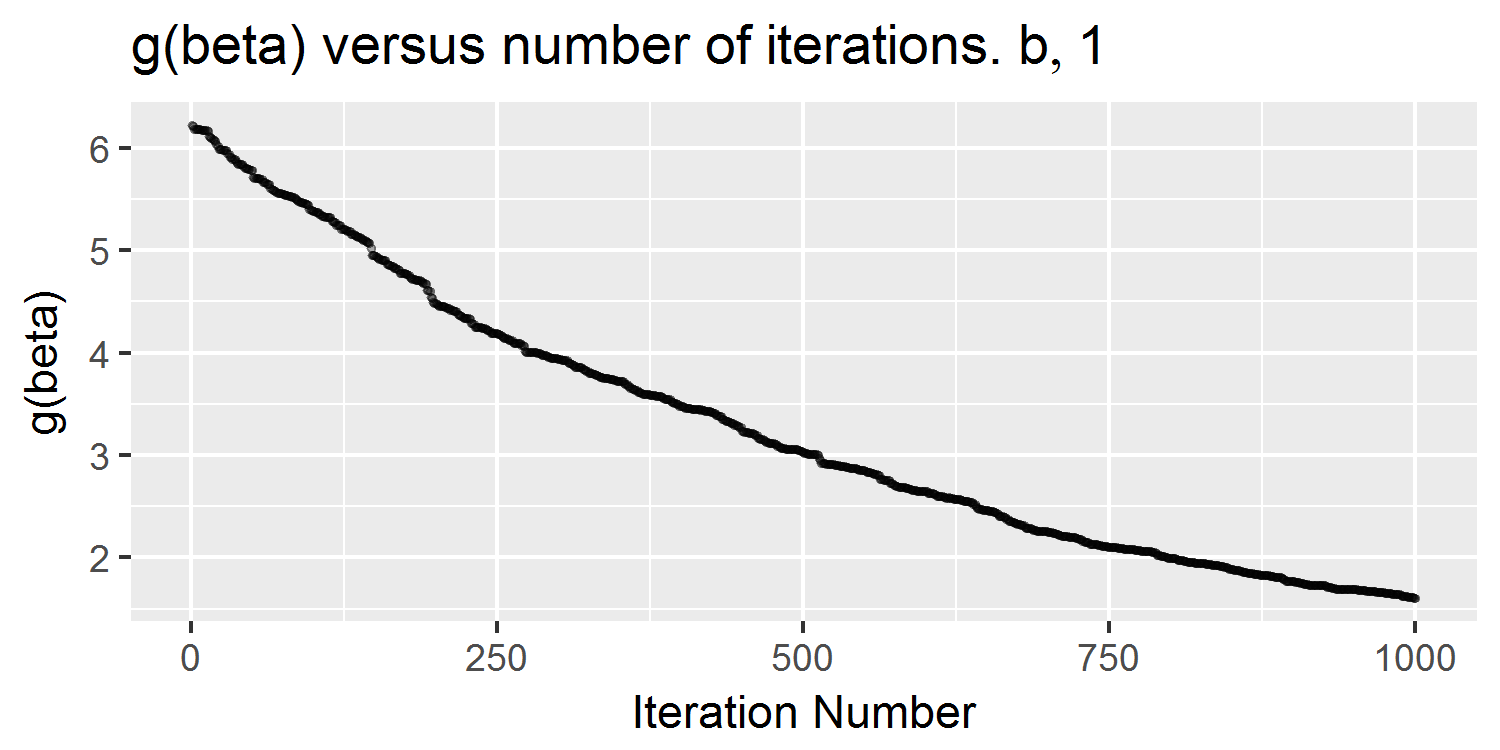
\includegraphics{../R/P2_Plot1}
	\end{center}

    We can see that with almost 1000 iterations the algorithm keeps looking for an optimal value of the loss function. Convergence is not fast and is not apparent that it has reached the minimum.
  ~\\
  
\part
\item Please draw three plots with $b=10,25,100$ for the value of objective function $g(\beta)$ versus the number of iterations to demonstrate the convergence.
~\\

\solution
~\\

We obtain the following three plots for $b=10,25,100$:

\begin{center}
	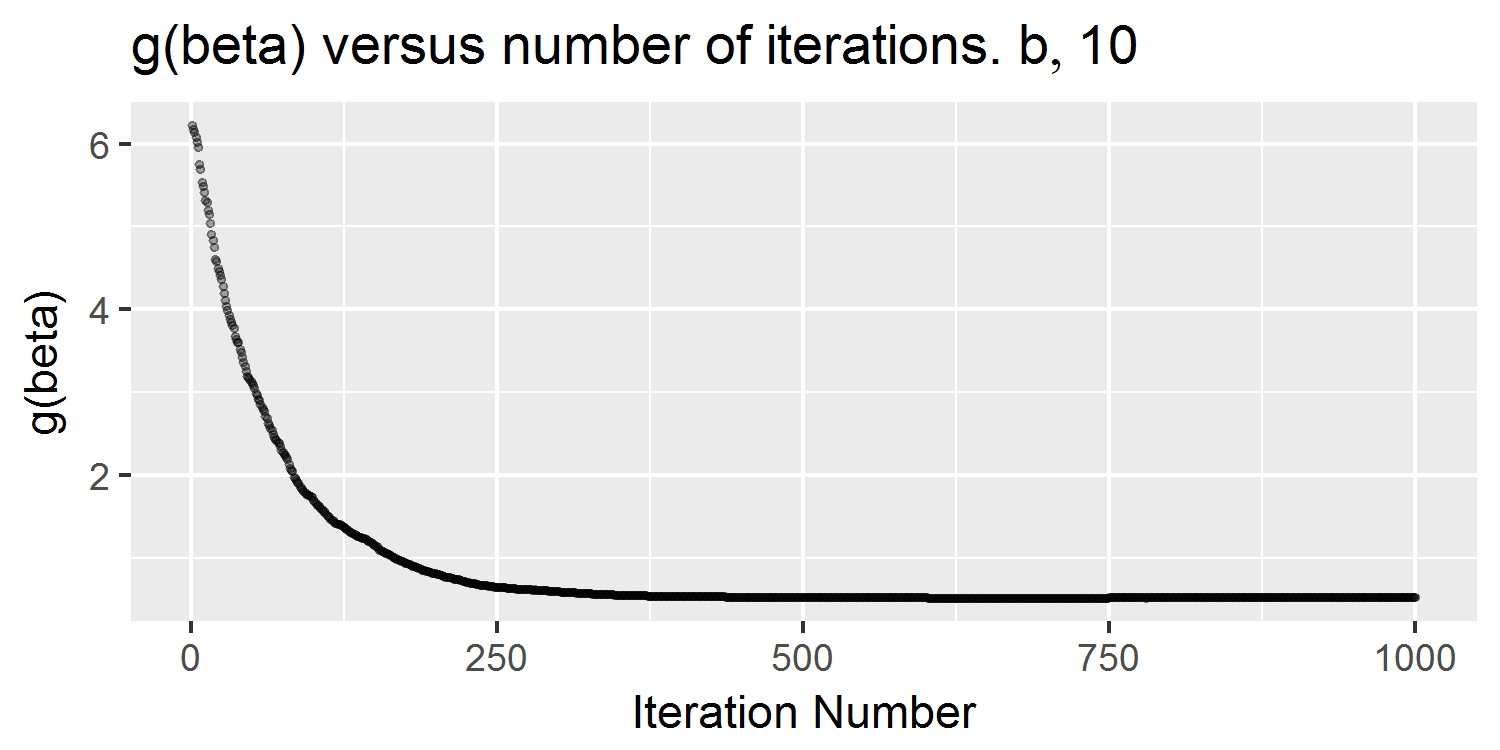
\includegraphics{../R/P2_Plot10}
	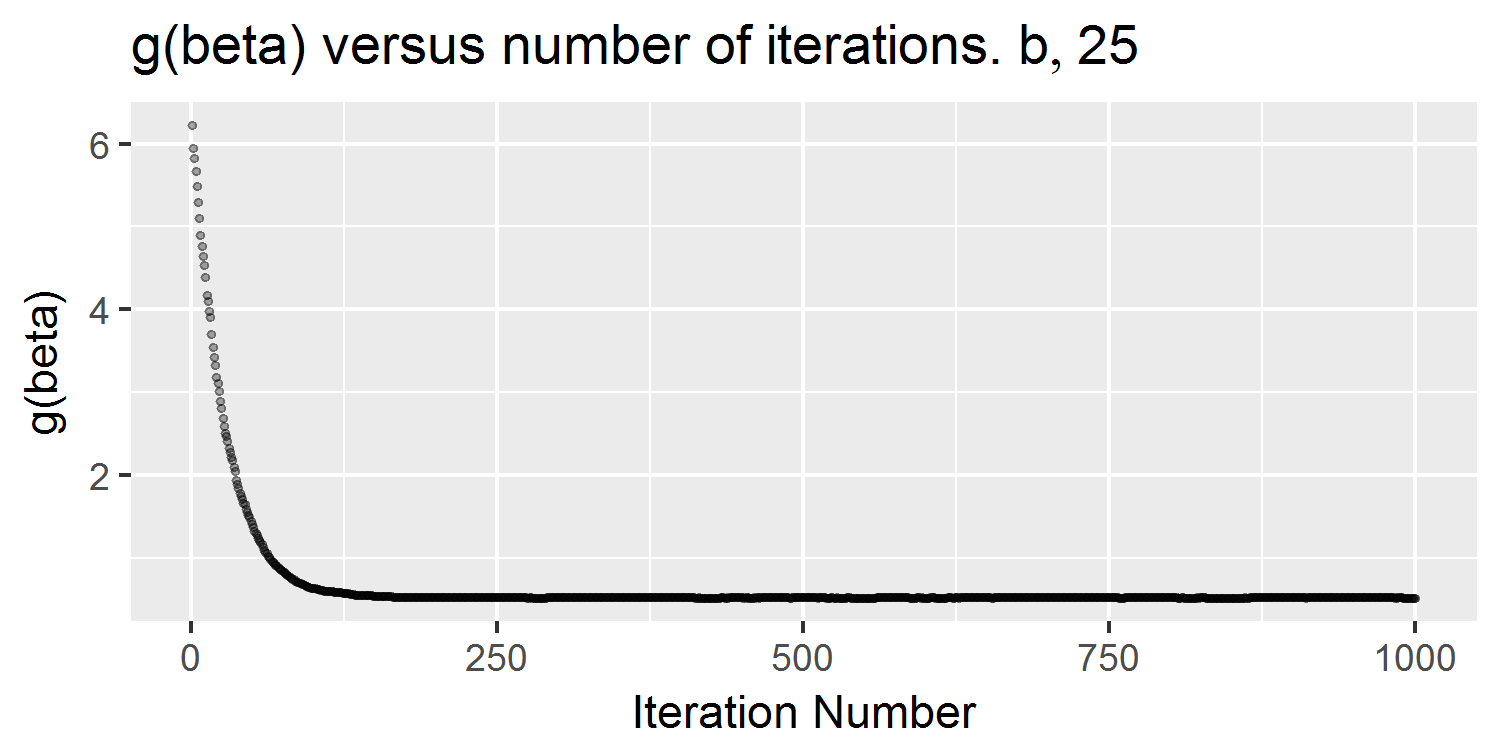
\includegraphics{../R/P2_Plot25}
	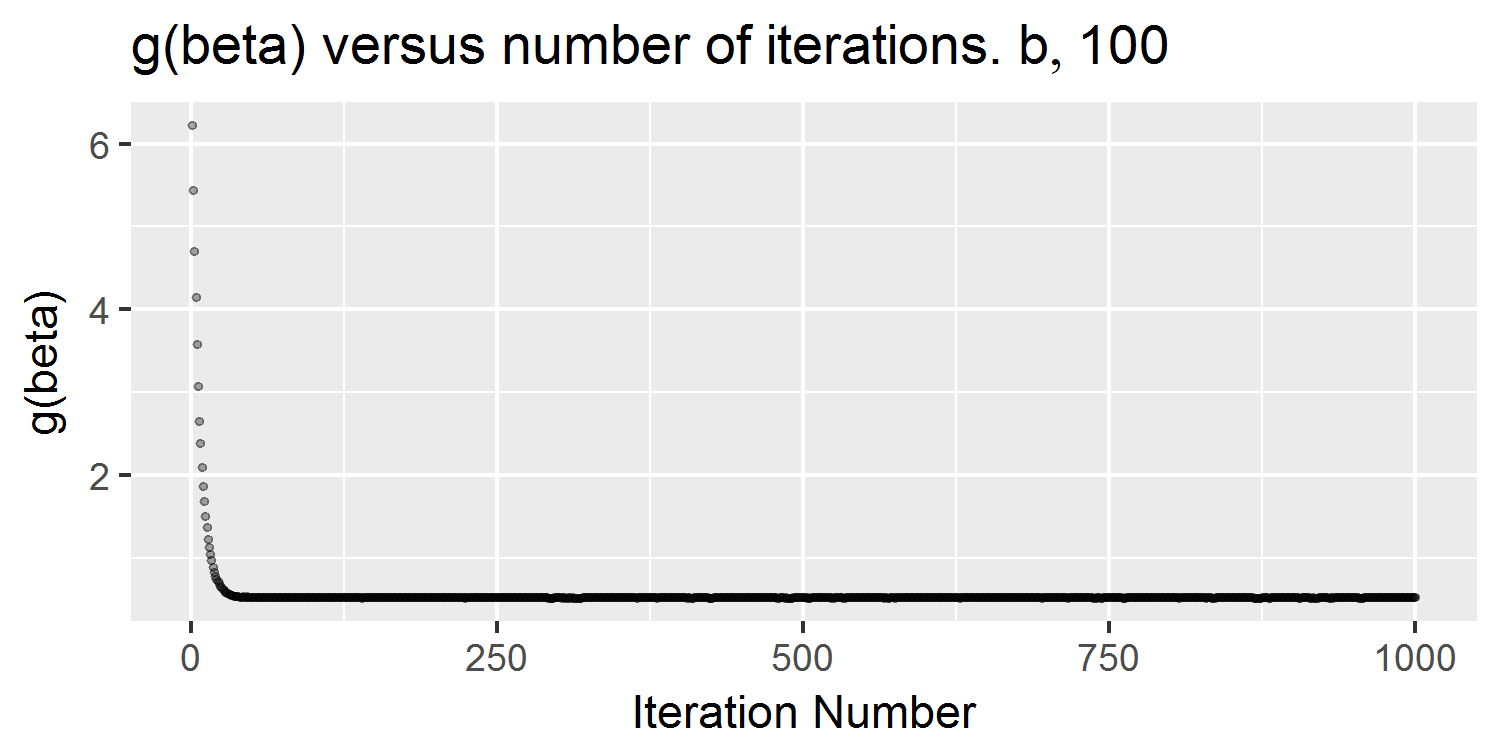
\includegraphics{../R/P2_Plot100}
\end{center}

We can see that as $b$ increases the algorithm converges faster. Almost 250 iterations for $b=10$, 100 iterations for $b=25$ and about 20 iterations for $b=100$.
    
\part
\item Please compare the result $\beta^*$ returned by your algorithm with the true $\beta$ by computing the mean squared error $\|\beta^* - \beta \|_2^2/30$.
~\\

\solution
~\\

The MSE for each $b$ are:

\begin{center}
	\begin{tabular}{||c c||} 
		\hline
		Algorithm & MSE \\ [0.5ex] 
		\hline\hline
		Stochastic Gradient Descent (b=1) & 0.0021607 \\ 
		\hline
		Mini-batch Stochastic Gradient Descent (b=10) & 0.0000590 \\
		\hline
		Mini-batch Stochastic Gradient Descent (b=25) & 0.0000656  \\
		\hline
		Mini-batch Stochastic Gradient Descent (b=100) & 0.0000310 \\
		\hline
	\end{tabular}
\end{center}

The larger the $b$ the smaller is the MSE. Is not only converging faster but we get better results for larger batches.
   
\end{homeworkProblem}

\pagebreak

\begin{homeworkProblem}
	\paragraph{Online Principal Component Analysis.}
	~\\
	
	\part
	\item Please draw a plot for $dist(w_i,v)$ versus number of iterations, where $w_i$ is the output of Oja's algorithm at $i$th iteration and $v$ is the true top eigenvector of $\Sigma$.
	~\\

	\solution
		~\\
	
	Oja's algorithm with step size $\eta_i = 1/100$ constant for all iteration seems to have a fast convergence but it has a jagged looking plot, meaning that with each constant step it seems to get away and closer at each iteration.
	
	~\\
	The final similarity measure $dist(w_n,v)$ is 0.007513874.
		
		\begin{center}
			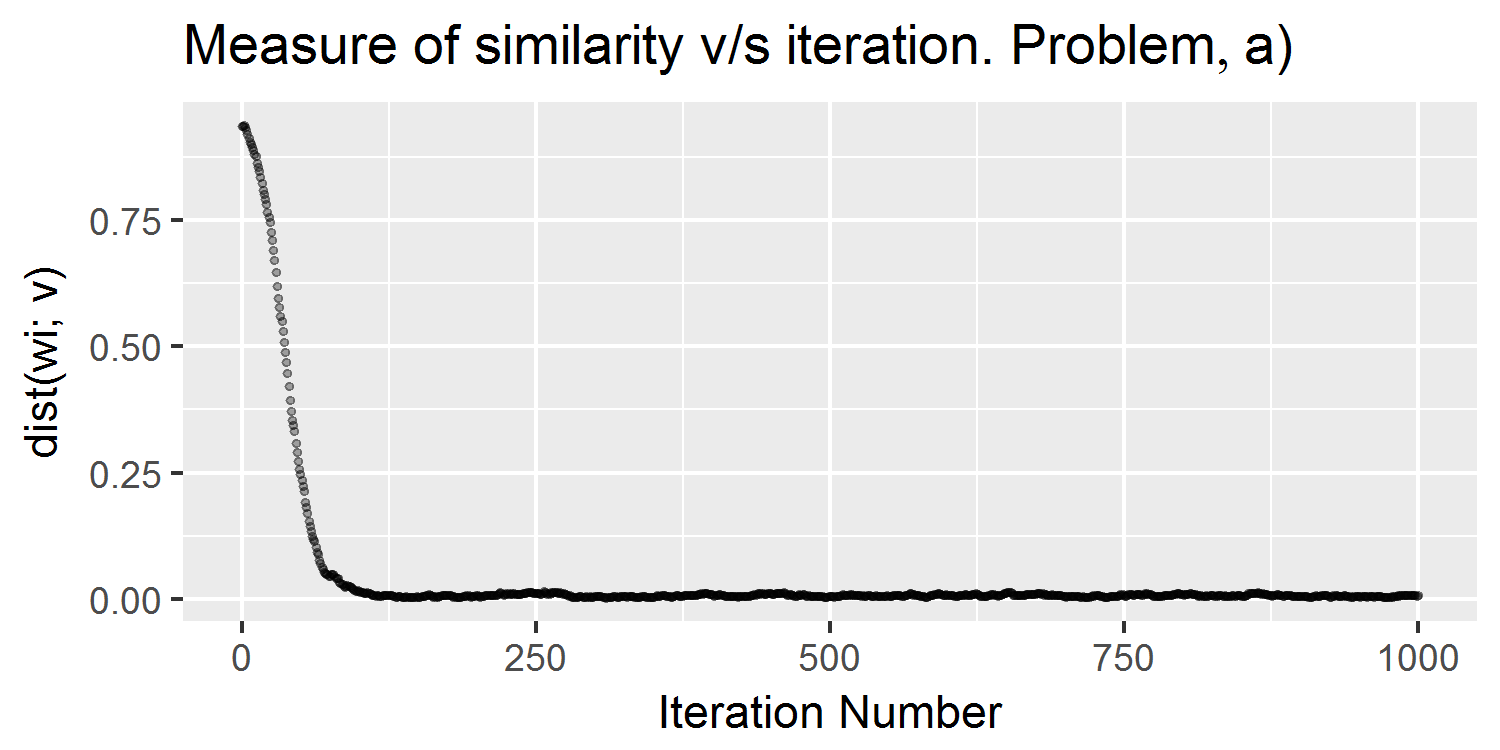
\includegraphics{../R/P3_Plota)}
		\end{center}
		
		\part
	\item Setting decreasing step sizes $\eta_i = 1/(100+i)$ at $i$th iteration. Please draw a plot for $dist(w_i,v)$ versus number of iterations..
	~\\
	
	\solution
	~\\
	When we use a variable step size $\eta_i = 1/(100+i)$ at each $i$th iteration the final similarity measure $dist(w_n,v)$ is 0.0006637931. Almost 10 times better accuracy than the previous result. Even though the convergence is slower, we have a smoother plot that converges to a more precise eigenvector $v$.

	\begin{center}
		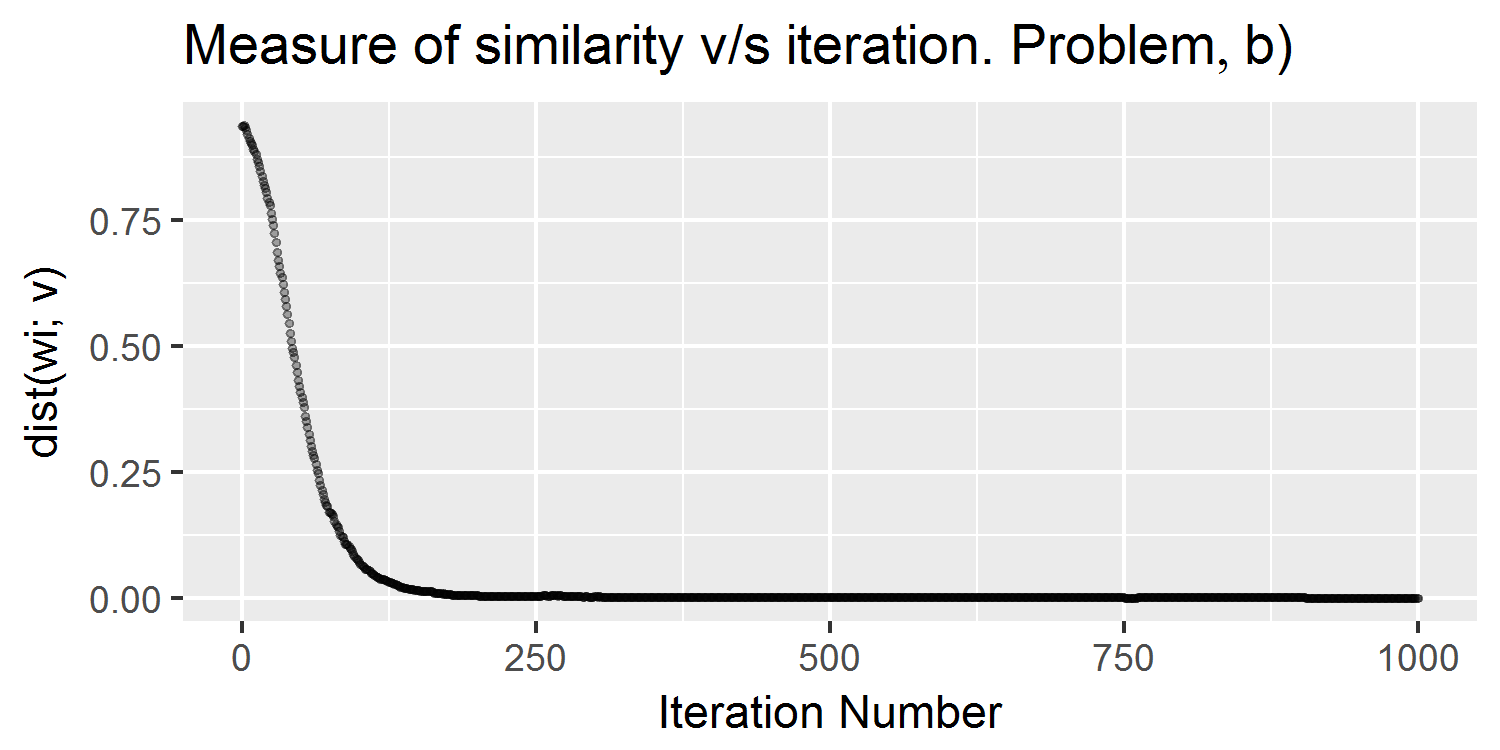
\includegraphics{../R/P3_Plotb)}
	\end{center}

\end{homeworkProblem}

\end{document}
